In this exercise, I analyze the performance of two bandit algorithms, a modified version of UCB1 and EXP3, under two different scenarios. First, I compare their performance in a standard i.i.d.\ environment where the best arm has a bias of $\mu^* = 0.5$ and the suboptimal arms have mean $\mu^*-\Delta$, with $\Delta\in\{0.25,0.125,0.0625\}$, and the number of arms $K\in\{2,4,8,16\}$. Second, I design a worst-case adversarial scenario to ``break'' UCB1, showing that even though UCB is robust in many cases, it can be forced to perform poorly under a specifically crafted reward sequence. In contrast, EXP3 (designed for adversarial settings) adapts much better.

\subsection*{Normal Comparison (IID Setting)}

In the i.i.d.\ experiments the modified UCB1 algorithm is used with the bonus term:
\[
\text{bonus} = \sqrt{\frac{\log t}{n_a}},
\]
where $n_a$ is the number of times arm $a$ has been played and $t$ is the current time step. The EXP3 algorithm uses a time-varying learning rate
\[
\eta_t = \sqrt{\frac{\ln K}{t \, K}}.
\]
Below is the code snippet for the EXP3 algorithm that was used:

\begin{lstlisting}
def run_exp3(T, means, nonstationary=False, worst_case=False, epsilon=0.01):
    n_arms = len(means)
    best_mean = np.max(means)  # Note: This may lead to negative regret initially
    regrets = np.zeros(T)
    cumulative_regret = 0.0
    L = np.zeros(n_arms)  # cumulative losses for each arm

    for t in range(T):
        eta_t = np.sqrt(np.log(n_arms) / ((t+1) * n_arms))
        L_min = np.min(L)
        w = np.exp(-eta_t * (L - L_min))
        p = w / np.sum(w)
        chosen_arm = np.random.choice(n_arms, p=p)
        
        if nonstationary and worst_case:
            reward = adversarial_reward(t, chosen_arm, T, epsilon)
        elif nonstationary:
            if chosen_arm == 1 and t >= T/2:
                reward = bernoulli_sample(0.0)
            else:
                reward = bernoulli_sample(means[chosen_arm])
        else:
            reward = bernoulli_sample(means[chosen_arm])
        
        cumulative_regret += (best_mean - reward)
        regrets[t] = cumulative_regret
        
        loss = (1 - reward) / max(p[chosen_arm], 1e-12)
        L[chosen_arm] += loss

    return regrets
\end{lstlisting}

\begin{figure}[H]
  \centering
  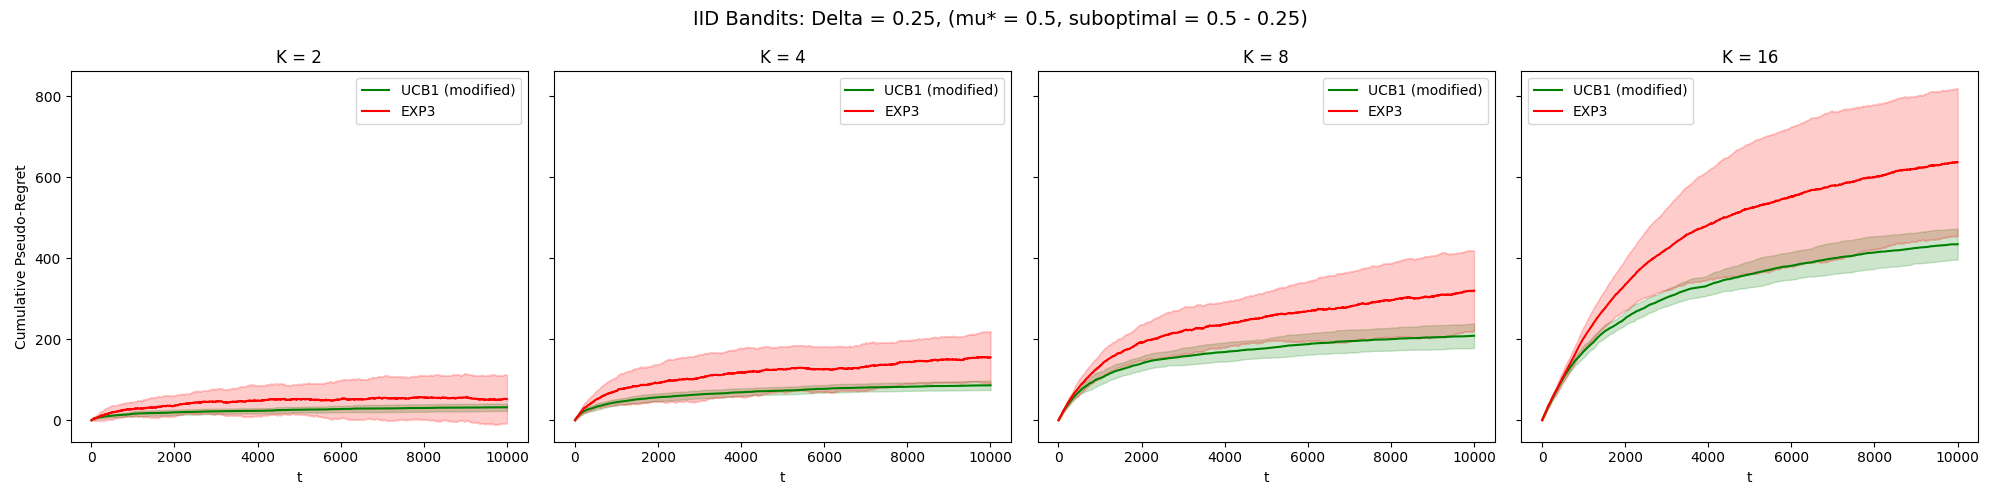
\includegraphics[width=1\textwidth]{Code/iid_experiment_delta_0_25.png}
  \caption{Cumulative pseudo-regret for $\Delta=0.25$, best arm $\mu^* = 0.5$, suboptimal arms = $0.5 - 0.25$. We compare UCB1 (modified) and EXP3 over $K=2,4,8,16$.}
\end{figure}

\begin{figure}[H]
  \centering
  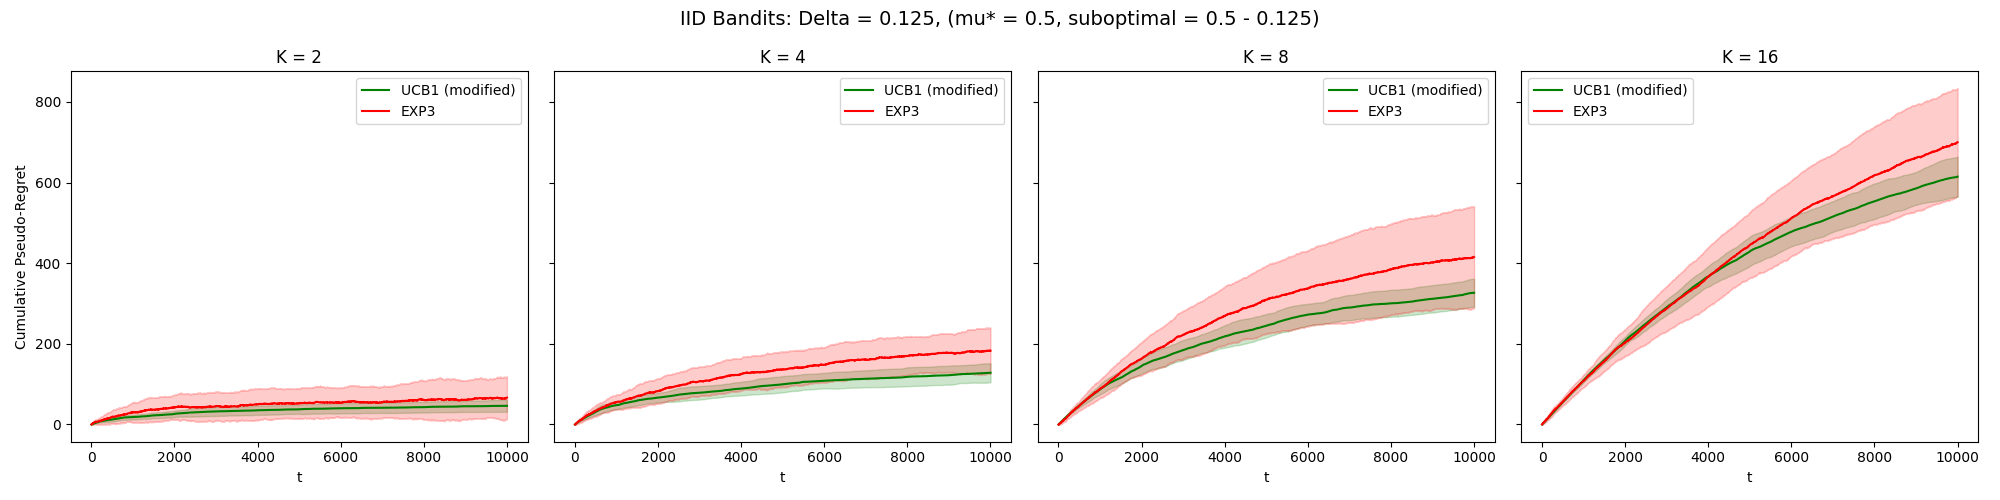
\includegraphics[width=1\textwidth]{Code/iid_experiment_delta_0_125.png}
  \caption{Cumulative pseudo-regret for $\Delta=0.125$, best arm $\mu^* = 0.5$, suboptimal arms = $0.5 - 0.125$. We compare UCB1 (modified) and EXP3 over $K=2,4,8,16$.}
\end{figure}

\begin{figure}[H]
  \centering
  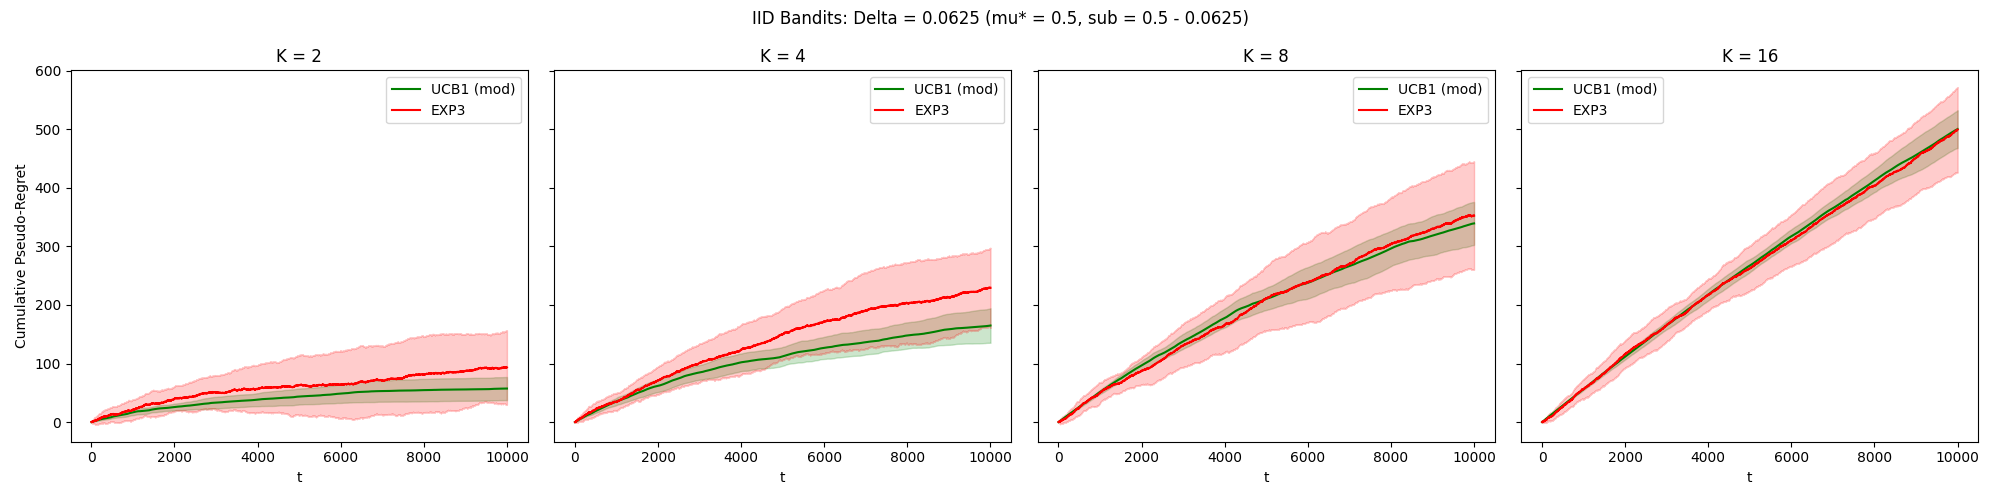
\includegraphics[width=1\textwidth]{Code/iid_experiment_delta_0_0625.png}
  \caption{Cumulative pseudo-regret for $\Delta=0.0625$, best arm $\mu^* = 0.5$, suboptimal arms = $0.5 - 0.0625$. We compare UCB1 (modified) and EXP3 over $K=2,4,8,16$.}
\end{figure}

\bigskip
\textbf{Discussion:} \\
The plots above illustrate the cumulative pseudo-regret for both algorithms in the i.i.d.\ setting. It can be observed that:
\begin{itemize}
    \item The modified UCB1 algorithm performs overall better in the i.i.d.\ environment, and this advantage is especially noticeable for large $K$ and large $\Delta$.
    \item EXP3 sometimes starts with negative regret because its pseudo-regret is computed as $(\text{best\_mean} - \text{reward})$, and early on the reward can exceed the nominal best mean.
    \item The variance (or standard deviation) of EXP3's regret is often larger, as indicated by the wider confidence bands, reflecting more variability in its performance across runs.
\end{itemize}

\subsection*{Worst-Case Adversarial Setting (Breaking UCB)}

To force UCB1 to perform poorly, I designed a worst-case adversarial scenario. The adversarial reward schedule is defined as follows:
\begin{itemize}
    \item For $t < T/2$:
    \begin{itemize}
       \item Arm 0: reward = 0.
       \item Arm 1: reward = 1.
    \end{itemize}
    \item For $t \ge T/2$:
    \begin{itemize}
       \item Arm 0: reward = 1.
       \item Arm 1: reward = 1 with probability $\epsilon$, and 0 otherwise.
    \end{itemize}
\end{itemize}
This reward structure is chosen so that UCB1, which initially observes high rewards for arm 1, builds up a high empirical average and large sample count on that arm. When the reward pattern switches, UCB1 continues to favor arm 1 and thus suffers nearly linear regret. Meanwhile, EXP3 adapts quickly to the change.

Below is the code snippet for the adversarial reward function and the corresponding experiment:

\begin{lstlisting}
def adversarial_reward(t, arm, T, epsilon=0.01):
    if t < T/2:
        return 1 if arm == 1 else 0
    else:
        if arm == 0:
            return 1
        else:
            return 1 if np.random.rand() < epsilon else 0
\end{lstlisting}

\begin{lstlisting}
def run_experiment_break(T=10000, n_runs=20, epsilon=0.01):
    all_regrets_ucb = np.zeros((n_runs, T))
    all_regrets_exp3 = np.zeros((n_runs, T))
    means = [0.5, 0.9]  # reference means, but actual rewards come from adversarial_reward
    
    for r in range(n_runs):
        reg_ucb = run_ucb(T, means, version='modified', nonstationary=True,
                          worst_case=True, epsilon=epsilon)
        all_regrets_ucb[r,:] = reg_ucb
        
        reg_e3 = run_exp3(T, means, nonstationary=True, worst_case=True, epsilon=epsilon)
        all_regrets_exp3[r,:] = reg_e3

    % (Plotting code is omitted here for brevity)
    return all_regrets_ucb, all_regrets_exp3
\end{lstlisting}

\begin{figure}[H]
    \centering
    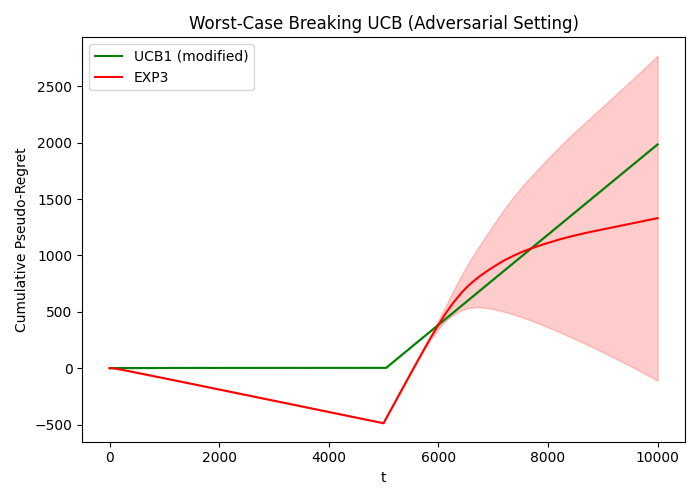
\includegraphics[width=1\textwidth]{Code/break_experiment_worst_case.png}
    \caption{Worst-case adversarial scenario designed to break UCB1 (modified). Arm 1 is good for $t < T/2$, then flips, forcing UCB1 to suffer linear regret while EXP3 adapts faster.}
\end{figure}

\bigskip
\textbf{Discussion:} \\
In this adversarial setting:
\begin{itemize}
    \item For $t < T/2$, arm 1 is heavily favored, so UCB1 builds a high empirical mean for arm 1.
    \item When $t \ge T/2$, the rewards flip, but UCB1 is slow to update its estimates and continues to select arm 1, which now almost always returns 0.
    \item EXP3, however, adjusts its probabilities based on the observed losses and quickly shifts its preference to arm 0.
\end{itemize}

It is noteworthy that breaking UCB is considerably harder than breaking Follow-The-Leader (FTL). In previous assignments, a simple repeating sequence of 0's and 1's was enough to break FTL via deterministic tie-breaking. However, UCB's exploration bonus and reliance on empirical means make it more robust, and for this reason a specifically crafted adversarial sequence (as shown above) is necessary to force it into linear regret.